%&pdflatex
\documentclass[1p]{elsarticle}

\usepackage{lineno,hyperref}
\usepackage{amsmath, amssymb, amscd, amsthm, amsfonts}
\usepackage{mathtools}

\DeclareMathAlphabet{\mathpzc}{OT1}{pzc}{m}{it}

\modulolinenumbers[5]

\setlength{\parskip}{.4em} 

\DeclarePairedDelimiter\ceil{\lceil}{\rceil} \DeclarePairedDelimiter\floor{\lfloor}{\rfloor}

\newtheorem{theorem}{Theorem}
\newtheorem{lemma}[theorem]{Lemma}
\newtheorem{conjecture}[theorem]{Conjecture}
\newtheorem{corollary}[theorem]{Corollary}
\newtheorem{example}[theorem]{Example}

\newcommand{\NPZ}{\ooalign{$Z$\cr\hfil\rule[.8ex]{.3em}{.09ex}\hfil\cr}}
\newcommand{\zn}{\ooalign{$z$\cr\hfil\rule[.5ex]{.2em}{.08ex}\hfil\cr}}

\journal{Discrete Applied Mathematics}

\bibliographystyle{elsarticle-num}

\begin{document}
	
	\begin{frontmatter}
		
		\title{Zombie number of the Cartesian product of graphs}
		
		
		%% or include affiliations in footnotes:
		\author{Ali Keramatipour}
		\ead{alikeramatipour@ut.ac.ir}
		
		\author{Behnam Bahrak\corref{correspondingauthor}}
		\cortext[correspondingauthor]{Corresponding author}
		\ead{bahrak@ut.ac.ir}
		
		\address{School of Electrical and Computer Engineering, College of Engineering, University of Tehran, Tehran, Iran}
		
		\begin{abstract}
		{\it Zombies and Survivor} is a variant of the pursuit-evasion game {\it Cops and Robber(s)}, with the
		difference that zombies must always move closer to the survivor. The game is played on a simple graph by two
		players. The goal of the zombies is to catch the survivor while the survivor's objective is to avoid being
		captured. The {\it zombie number} of $G$, denoted as $\zn(G)$, is the minimum number of zombies required to
		capture a single survivor on $G$, no matter what moves the survivor makes. In this paper, we prove a conjecture
		by Fitzpatrick et al.\cite{Fitz16} about the zombie number of the {\it Cartesian product} of two graphs. This
		result provides a new proof for $\zn(Q_n) = \ceil*{\frac{2n}{3}}$. We also introduce a new problem regarding
		{\it capture time} in the Cartesian product of two graphs. At last, we study computational complexity of finding
		the zombie number of a graph $G$, with and without a limited {\it capture time}.
		\end{abstract}
		
		\begin{keyword}
			Cartesian Product of Graphs\sep Zombie Number\sep NP-Hard
		\end{keyword}
		
	\end{frontmatter}
	
\section{Introduction}\label{section-introduction}

The {\it Zombies and Survivor} game is played on a simple graph by two players (we only discuss connected graphs, proofs
can be easily modified for disconnected graphs). The deterministic version of this game \cite{Fitz16} is played as
follows. Initially, the zombie player has $\mathpzc{z}$ zombies and places them on the graph vertices. This initial
arrangement that zombie player chooses is essential for him to win.  Then the survivor player chooses one single vertex
which is the survivor's initial position. Starting with the zombie player, on each player's turn, the zombie player must
move each zombie to one of its adjacent vertices so that they get closer to the survivor, while the survivor player
either moves to an adjacent vertex or stays at his current location. Here lies the difference between {\it Zombies and
Survivor} and {\it Cops and Robber(s)} games, as in {\it Cops and Robber(s)} cops need not necessarily get closer to the
robber(s). They can either hold their current position, get closer, or further away from the robber(s). Although zombies
are not as intelligent as cops, they can still choose their path intelligently between the shortest paths. If any zombie
and the survivor ever occupy the same vertex, the survivor is captured and the zombie player wins. The zombie number of
a graph $G$, denoted as $\zn(G)$, is the minimum number of zombies required so that the zombie player can always capture
the survivor, no matter how survivor moves.

The Cartesian product $G \square H$ of two graphs $G$ and $H$, is a graph with vertex set of $V(G) \times V(H)$, where
vertices $(u_1 , u_2)$ and $(v_1 , v_2)$ are adjacent if and only if $u_1 = v_1$ and $ \{ u_2 , v_2 \} \in E_{H} $, or
$u_2 = v_2$ and $ \{u_1 , v_1 \} \in E_{G}$ \cite{West02}. Figure \ref{fig:p2} shows an example of the Cartesian product
of two graphs.

{\it Capture time} of a game \cite{Bonato09}, noted as $capt(G,\mathpzc{z})$, represents the maximum number of moves
that survivor can avoid being caught on a graph $G$, while the zombie player tries to catch survivor as quickly as
possible using $\mathpzc{z}$ zombies. If a survivor-win play exist, $capt(G,\mathpzc{z})$ goes to infinity.

\begin{figure}[h!]
	\centering
	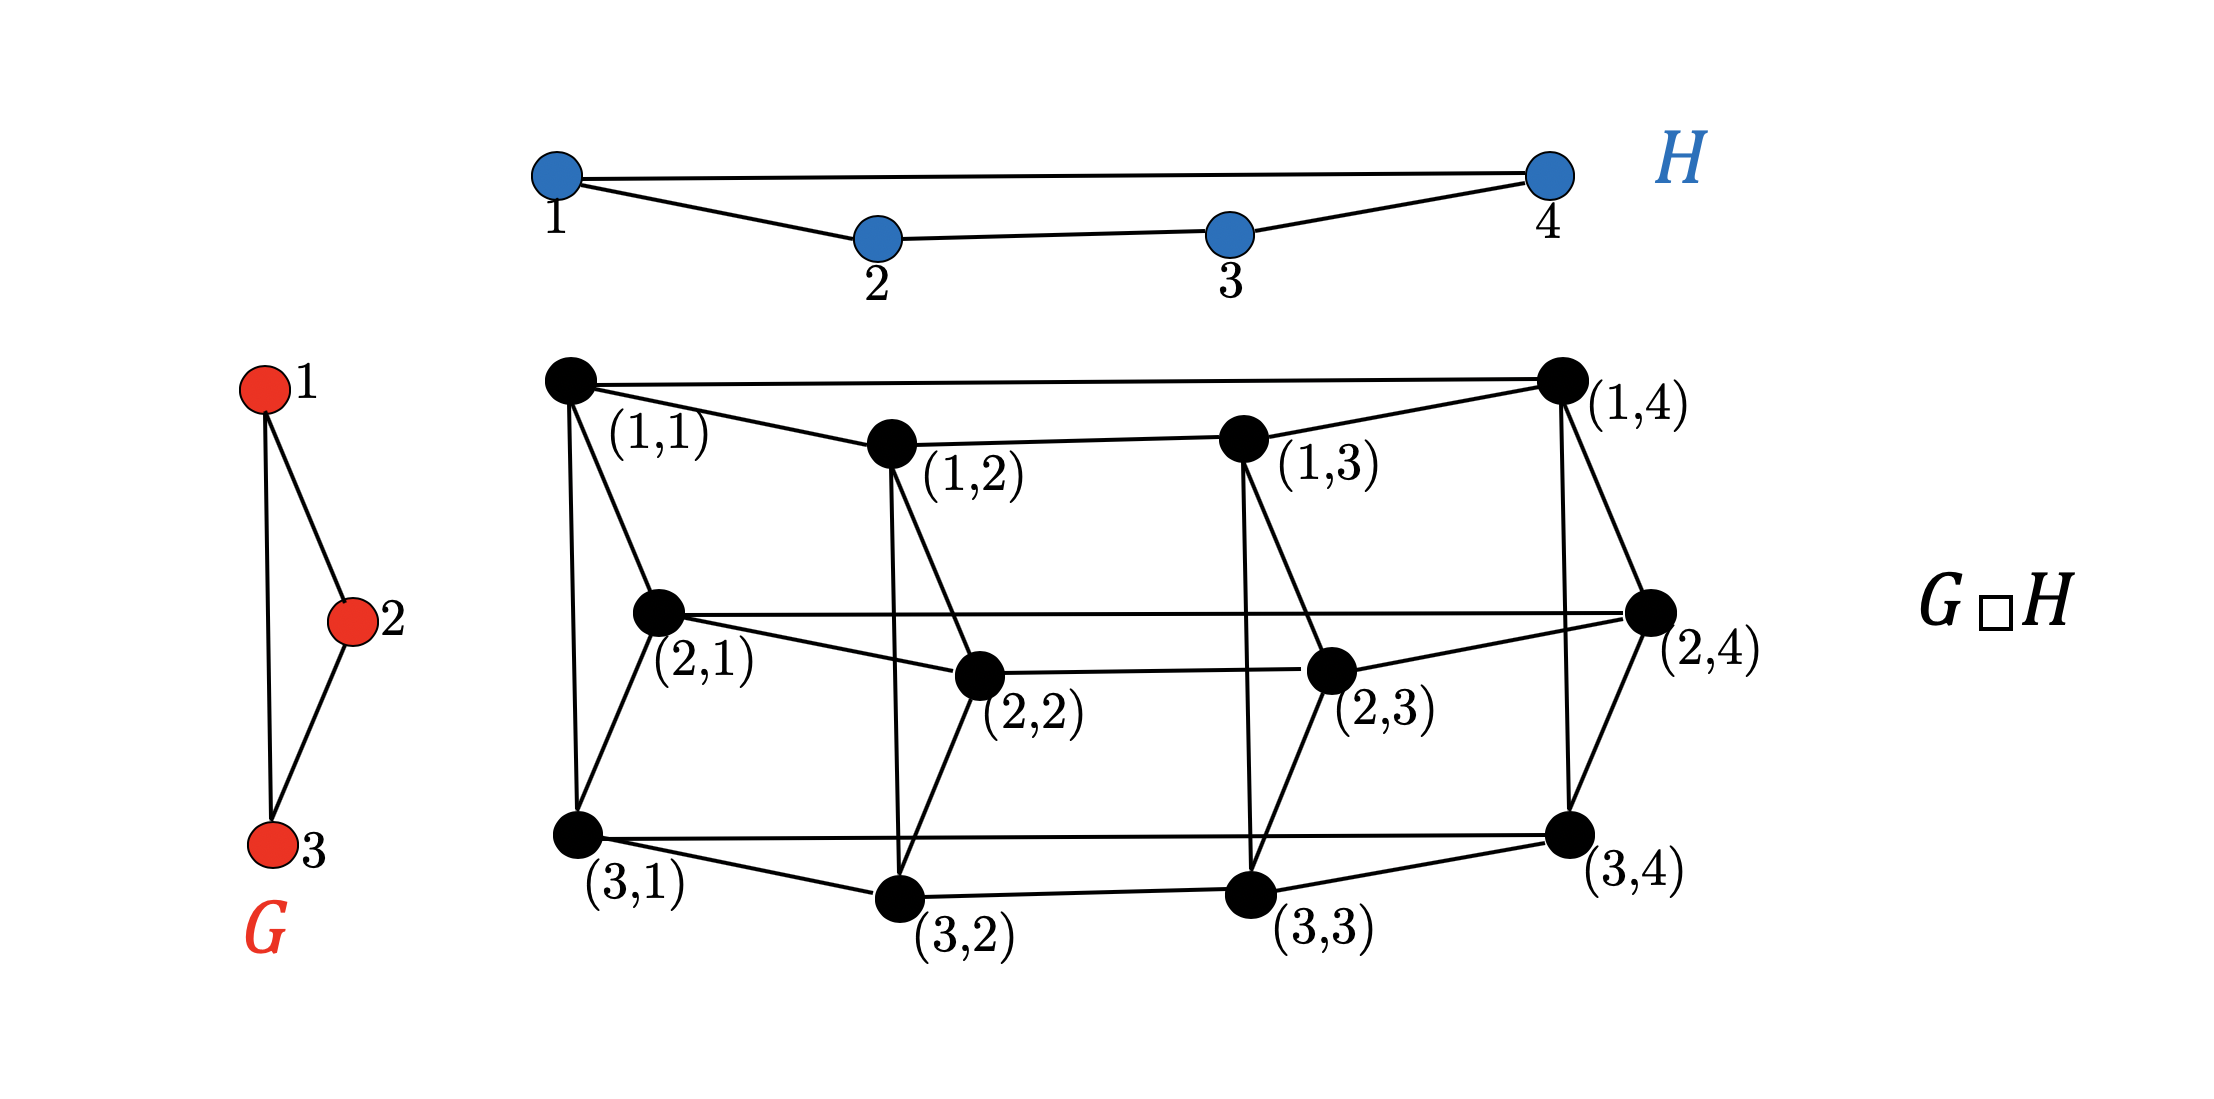
\includegraphics[width=0.9\linewidth]{fig/CpWest.png}
	\caption{$C_3 \square C_4$ an example of the Cartesian product}
	\label{fig:p2}
\end{figure}

Our contributions can be summarized as follows:

1) In \cite{Fitz16}, Fitzpatrick et al. conjectured that $\zn(G \square H) \leq \zn(G) + \zn(H)$. In section \ref{conj-proof}, we prove this conjecture and
use it to show that $\zn(Q_n) = \ceil*{\frac{2n}{3}}$. 

2) In section \ref{capturetime}, we provide a new bound on {\it capture time} of {\it zombies and survivor} game played on the Cartesian
product of two graphs. 

3) We introduce a variation of {\it zombies and survivor} game, in which the zombie player is restricted to winning in a
limited number of moves in section \ref{np-capturetime}, and prove it belongs to {\it NP-Hard} class of problems.

4) In section \ref{np-zombienumber}, we prove that the original {\it zombies and survivor} game belongs to {\it NP-Hard} class
of problems.


\section{Zombie number of the Cartesian product of two graphs}\label{conj-proof}

To prove $\zn(G \square H) \leq \zn(G) + \zn(H)$, we show that $\zn(G) + \zn(H)$ zombies are enough for the zombie player to
capture the survivor on $G \square H$.

To explain the proof we first need to define some notation. Assume $H$ and $G$ have $m$ and $n$ vertices,
respectively. 

For $1 \leq i \leq m$, define $G_i$ to be the subgraph induced by vertices $(u,v = i)$. Similarly, for $1 \leq j \leq
n$, define $H_{j}$ to be the subgraph induced by vertices $(u = j,v)$.

In the Cartesian product of $G$ and $H$, each $G_{i}$ $(1 \leq i \leq m)$ is isomorphic to $G$, and each $H_{j}$ $(1
\leq j \leq n)$ is isomorphic to $H$. Also the common vertex between $G_{i}$ and $H_{j}$ is $(j,i)$, and $(x,y)$ is the
vertex where the survivor is located. Figure \ref{fig:p1} illustrates these definitions.

A {\it G-edge} is an edge in one of the $G_{i}$s and an {\it H-edge} is an edge in one of the $H_{j}$s. A {\it G-move}
is a move made on a {\it G-edge}. Similarly, an {\it H-move} is a move made on an {\it H-edge}. If the survivor decides
to remain in its current vertex, this move is considered both a {\it G-move} and an {\it H-move}. 

Define $dist_I(j,k)$ to be the distance between vertices $j$ and $k$ on a graph $I$. Define the length of a path $P$ to be $len(P)$. 

For vertex $(u,v)$, define its $G$-equivalent vertex to be vertex $u \in G$, and its $H$-equivalent vertex, to be vertex
$v \in H$. $G$-equivalent graph is a graph where each zombie and the survivor is put on its $G$-equivalent vertex.
$H$-equivalent graph is defined in the same way.


\begin{figure}[h!]
	
	\centering
	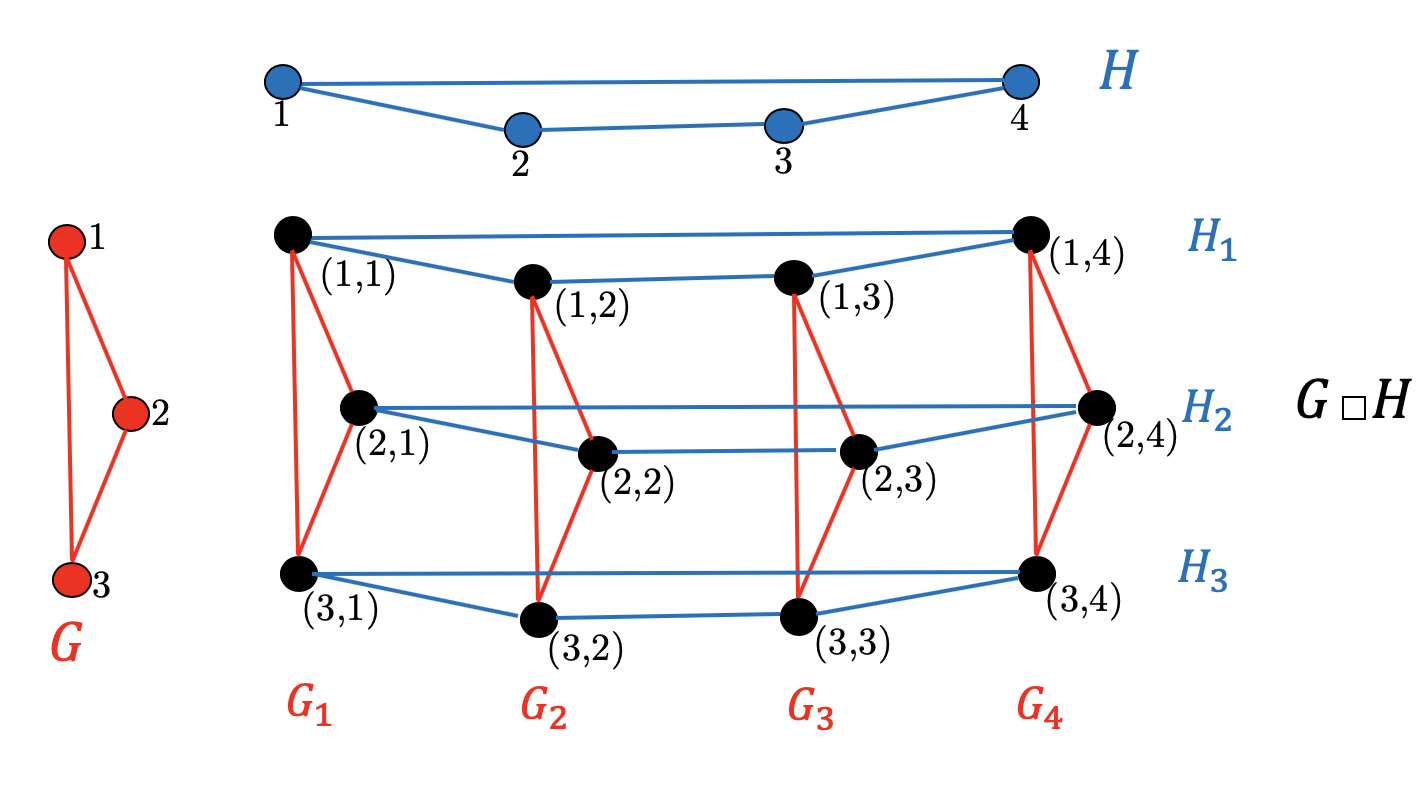
\includegraphics[width=0.9\textwidth]{fig/cp3.png}
	\caption{$G \square H$, $G_i$s, and $H_i$s.}
	\label{fig:p1}
\end{figure}



\begin{lemma} \label{shortestpathlemma}
	$dist_{G \square H}((x,y),(u,v)) = dist_G(x,u) + dist_H(y,v)$.
\end{lemma}
\begin{proof}
	Since there is a path from $(x,y)$ to $(x,v)$ with length $dist_H(y,v)$ and a path from $(x,v)$ to $(u,v)$ of length
	$dist_G(x,u)$, we only need to prove there can be no path with length less than $dist_G(x,u) + dist_H(y,v)$. Suppose
	not, this path uses some {\it G-edge}s and some {\it H-edge}s. If a {\it G-edge} is followed by an {\it H-edge} (or
	vice-versa), then we can swap these edges and still end up in the same vertex. For example, path $(u_1,v_1) \rightarrow
	(u_2,v_1) \rightarrow (u_2,v_2)$ ends up in the same vertex as path $(u_1,v_1) \rightarrow (u_1,v_2) \rightarrow
	(u_2,v_2)$. Since we can swap each two edges of different type, there is a path with {\it G-edge}s before {\it
	H-edge}s with the same length that has all {\it G-edge}s in $G_y$ and all {\it H-edge}s in $H_u$. Since this path
	has a length less than $dist_G(x,u) + dist_H(y,v)$, there must be an $x,u-$path in $G$, with length less than
	$dist_G(x,u)$, or a $y,v-$path in $H$, with length less than $dist_H(y,v)$, which is a contradiction. Thus the
	statement holds.
\end{proof}




\begin{theorem}
	\label{T2}
	$\zn(G \square H) \leq \zn(G) + \zn(H)$.
\end{theorem}

\begin{proof}
	We provide a winning strategy for the Cartesian product of $G$ and $H$ using $\zn(G)+\zn(H)$ zombies. First, we place
	$\zn(G)$ zombies, that have a winning strategy on a single $G$, $G_{a = 1}$ and call them {\it G-zombie}s. We do the
	same for $H_{b = 1}$ and call them {\it H-zombie}s.


	Consider one of the shortest paths between vertices $a$ (the index of $G$-subgraph shared by {\it G-zombie}s) and
	$y$ in $H$ and call it $p_H$. We also define $p_G$ in the same manner between $b$ and $x$.


	On each zombie turn, if $a \neq y$, each {\it G-zombie} will move along the $p_H$ path in its corresponding $H$
	subgraph. According to lemma \ref{shortestpathlemma}, since zombies' and survivor's equivalents on $H$ are getting
	closer, thus their actual vertices on $G \square H$ are getting closer as well and this move is possible. Since they
	are all moving along similar paths (in their corresponding $H$-subgraphs) they will still share the same
	$G$-subgraph. Now consider when $a = y$, {\it G-zombie}s will play their winning strategy (that they had on a single
	$G$) in this case. This move is also possible since in $G$'s strategy, zombies would get closer to survivor on each
	turn. If $a = y$ and survivor makes an {\it H-move}, {\it G-zombie}s will maintain their positioning by mimicking
	the exact same move on their corresponding $H$. This means for those turns that $a=y$ holds, if we consider the
	$G$-equivalent graph between {\it G-zombie}s and the survivor, it is just like a simple game played on a single $G$.
	{\it H-zombie}s will follow the same strategy but in their corresponding environment.
	
	
	Suppose using this strategy the survivor wins, then the survivor must either do infinite {\it G-move}s or infinite
	{\it H-move}s. Without loss of generality, suppose the survivor makes infinite {\it H-move}s, we prove that this is
	not possible. After $len(p_G)$ number of {\it H-move}s, {\it H-zombie}s will get to $H_x$. Now for each {\it G-move}
	made by survivor and having zombies mimicking it, nothing changes in their $H$-equivalent graph. Since the survivor
	can do infinite {\it H-move}s and prevent being caught, it means that the survivor could also avoid being caught on
	a single $H$ which contradicts our assumption.
	
\end{proof}
An example for further understanding can be found at \ref{CartesianProductExample}.

\begin{corollary}
	\label{C3}
	$\zn(Q_{n}) \leq \ceil*{\frac{2n}{3}}$
\end{corollary}
\begin{proof}
	We prove this by using both induction and Theorem \ref{T2}. First note that the Cartesian product of
	hypercube graphs $Q_{m}$ and $Q_{n}$ is equal to $Q_{m+n}$. It is easy to see $\zn(Q_3) = 2$, $\zn(Q_2) = 2$, and
	$\zn(Q_1) = 1$. For $n > 3$, we consider $Q_n$ as the Cartesian product of $Q_3$ and $Q_{n-3}$. Using the induction
	base, we know that $\zn(Q_{n-3}) \leq \ceil*{\frac{2n - 6}{3}}$. According to Theorem \ref{T2}, $\zn(Q_n) \leq
	\zn(Q_{n-3}) + \zn(Q_3)$ and $\zn(Q_{n-3}) \leq \ceil*{\frac{2n - 6}{3}} = \ceil*{\frac{2n}{3}} - 2$, we can see that
	$\zn(Q_n) \leq \ceil*{\frac{2n}{3}}$.
\end{proof}

It is already proved that at least $\ceil*{\frac{2n}{3}}$ zombies are needed to capture one survivor on graph $Q_n$
(Theorem 16 of \cite{Fitz16}):

\begin{theorem}
	\label{T4}
	For each integer $n \geq 1$, $\zn(Q_n) \geq \ceil*{\frac{2n}{3}} $.
\end{theorem}

Combining {\it Corollary \ref{C3}} and {\it Theorem \ref{T4}} we can conclude that $\zn(Q_n) = \ceil*{\frac{2n}{3}}$.
This proves Conjecture 18 from \cite{Fitz16} which is already proved in \cite{Offner19} with a different method. 
	

\section{Capture time in Cartesian product of graphs}\label{capturetime}
	
	Let $rad(G)$ represent the length of $G$'s radius.
	\begin{theorem}
		\label{T5}
		$capt( G \square H, z_G + z_H ) < rad(G) + rad(H) + capt(G, z_G) + capt(H, z_H)$
	\end{theorem}
	\begin{proof}
		By using $z_G$ zombies as {\it G-zombie}s and $z_H$ zombies as {\it H-zombie}s, and having them follow the same
		set of moves provided in Theorem \ref{T2}, with the difference that initially $a$ and $b$ are centers of graphs
		$H$ and $G$. we show that survivor's {\it G-move}s cannot exceed $rad(H) + capt(G, z_G)$. With the same
		conclusion, it can be shown that {\it H-move}s cannot exceed $rad(G) + capt(H, z_H)$ as well.

		According to the definition of the radius of a graph, after at most first $radius(H)$ {\it G-move}s that
		survivor makes, $a = y$ holds. Now since for each {\it G-move} made from now on by survivor, {\it G-zombie}s can
		follow their strategy on a $G$ graph, and after at most $capt(G,z_G)$ {\it G-move}s, survivor will be captured. 
		
		Since each of survivor's moves is either a {\it G-move} or an {\it H-move} or both, after less than $rad(G) +
		rad(H) + capt(G, z_G) + capt(H, z_H)$ moves the survivor will be captured.
	\end{proof}
\section{Limited capture time zombie number problem is NP-Hard}\label{np-capturetime}
	A well known example of an NP-hard problem is the {\it dominating-set} problem in graph theory\cite{Hopcroft07}. A
	{\it dominating-set} for a graph $G$ is a subset $D$ of $V(G)$ such that every vertex not in $D$ is adjacent to at
	least one member of $D$. The domination number $\gamma(G)$ is the number of vertices in the smallest dominating-set
	for $G$.

	We define $Lc\zn(G,k)$ ({\it limited capture time zombie number}) as the minimum number of zombies needed so that
	zombie player is able to capture the survivor in at most $k$ moves on graph $G$. 

	Let $N_G[u]$ represent the closed neighborhood of $u$ in graph $G$.
	
	The $LC\NPZ_k$ problem is defined as below:
	{\newline}
	INSTANCE: A simple undirected graph $G = (V,E)$ and a positive integer $\mathpzc{z}$.
	{\newline}
	QUESTION: Is $Lc\zn(G,k) \leq \mathpzc{z}$ ?
	{\newline}
	{\newline}
	The dominating-set problem is defined below:
	{\newline}
	INSTANCE: A simple undirected graph $G = (V,E)$ and a positive integer $d$.
	{\newline}
	QUESTION: Is $\gamma(G) \leq d$ ?

	\begin{theorem}
		$LC\NPZ_k$ $\in$ NP-Hard
	\end{theorem}
	\begin{proof}
		We prove this by reducing the dominating-set problem to $LC\NPZ_k$ in polynomial time.

		Consider $k$ to be an arbitrary positive integer. We construct a new graph $G'_k$ from $G$. Suppose $G$
		has $n$ vertices. For each $v \in V(G)$, we add $k-1$ new vertices $(v,1 \leq i < k)$ making a {\it new} path,
		$(v,(v,1),(v,2),...,(v,k-1))$ (as shown in figure \ref{fig:p7}). Creating $G'_k$ can be done in polynomial time.

		\begin{figure}[h!]
			\centering
			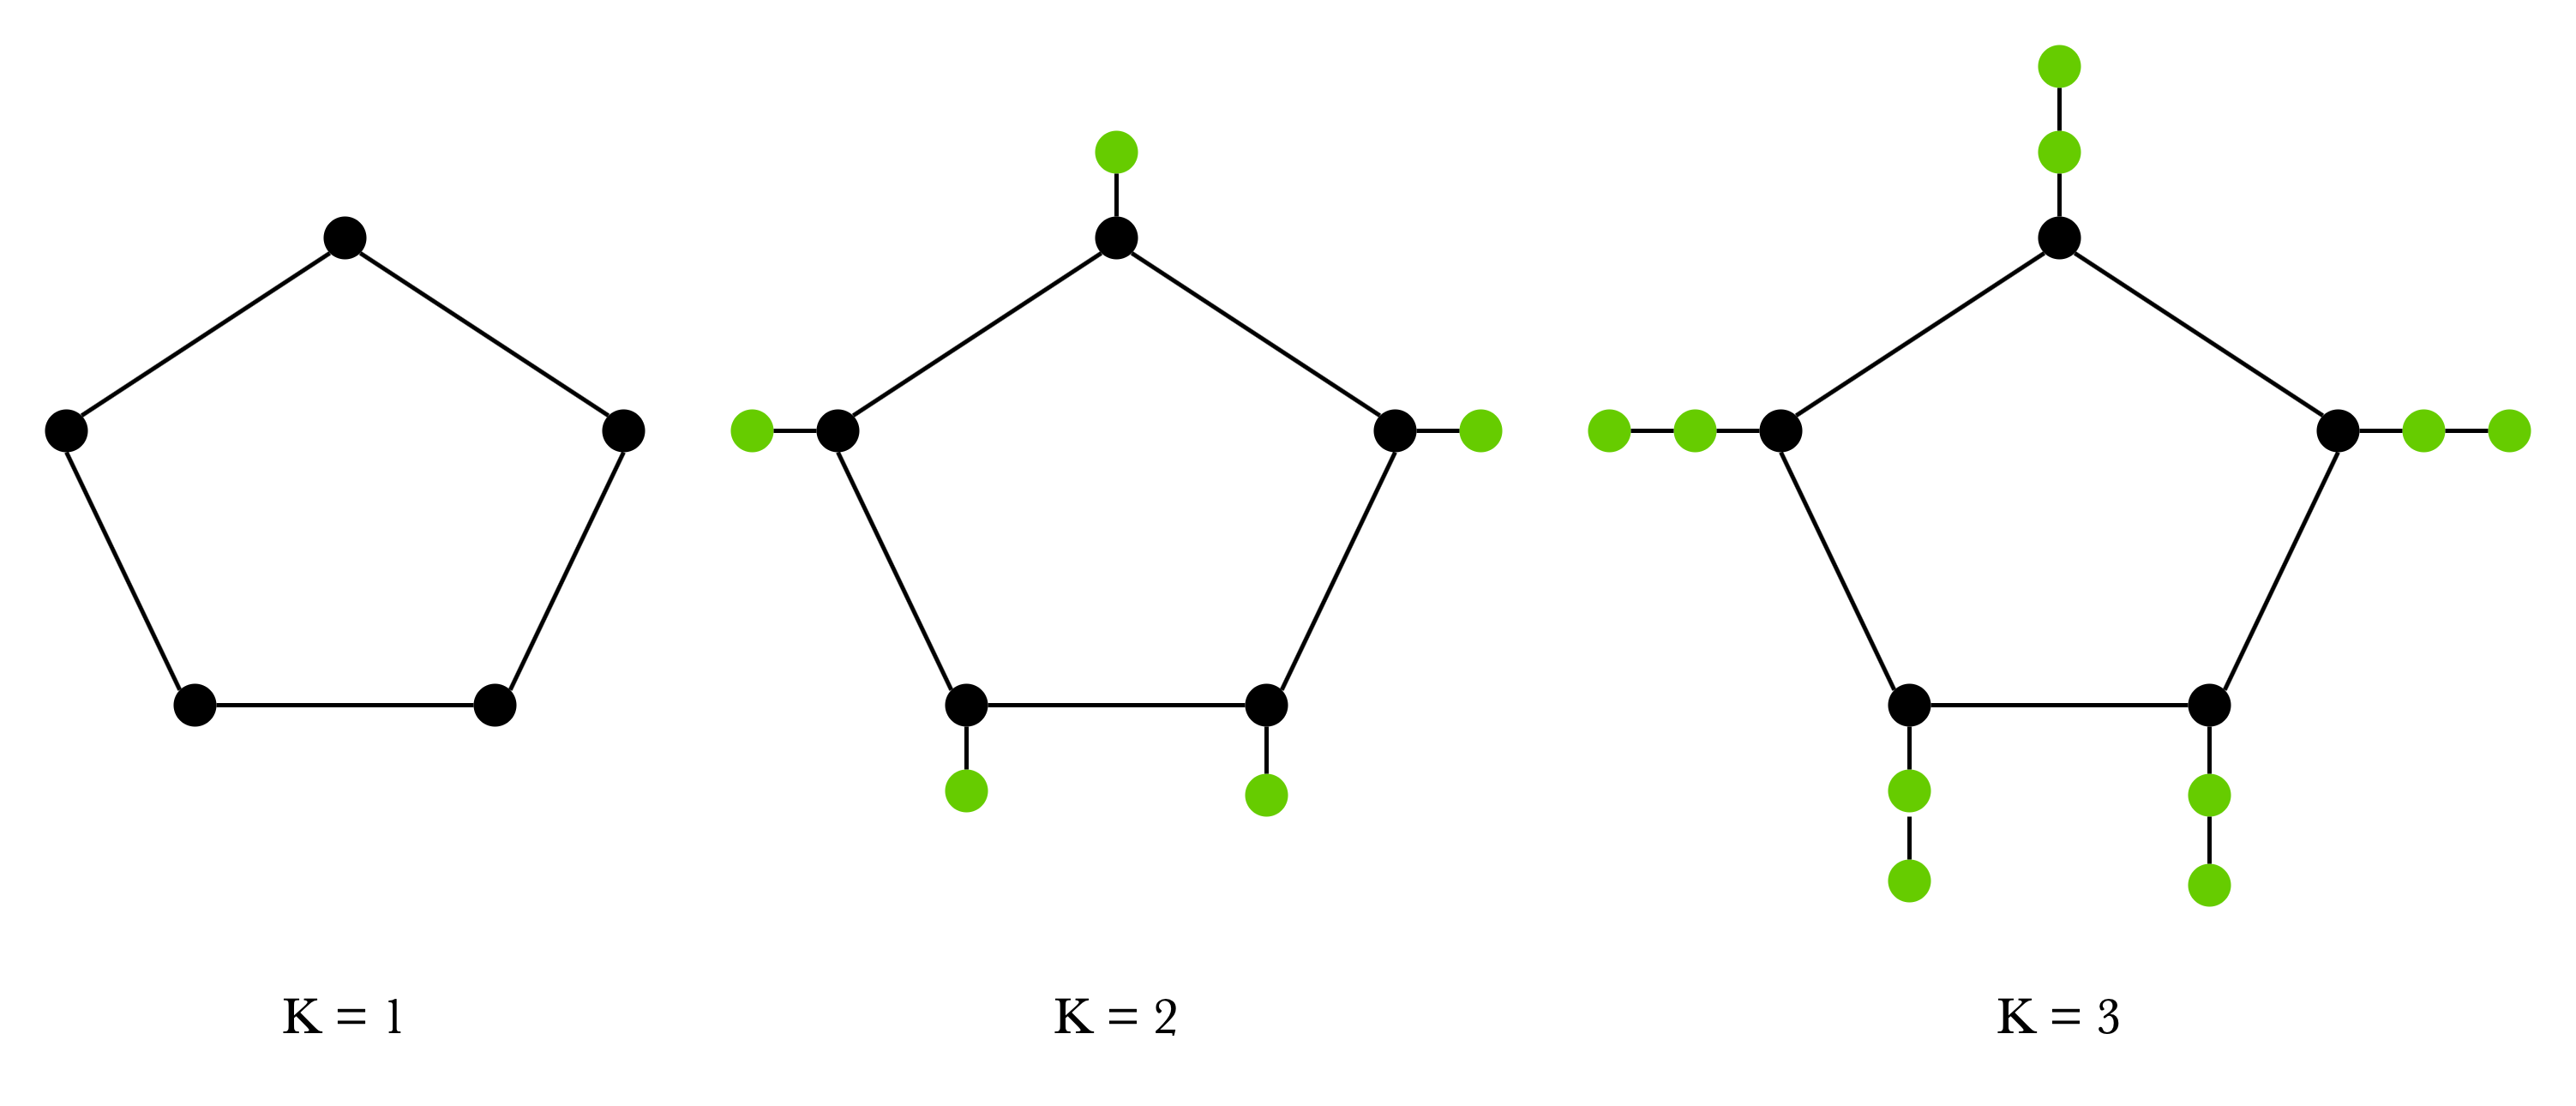
\includegraphics[width=0.9\linewidth]{fig/LCZ.png}
			\caption{$G'_k$ obtained from $G = C_5$ where for $k = 1,2,3$}
			\label{fig:p7}
		\end{figure}		


		We prove this by showing $Lc\zn(G'_k,k) = \gamma(G)$. Consider set $S'$ as zombies' initial vertices on $G'_k$,
		so that zombies are able to capture the survivor within $k$ moves. Let $S$ be the set of vertices $v \in V(G)$
		such that $v \in S'$ or $(v,i) \in S'$. If there is a vertex $u \in G$ not dominated by $S$, then there is no
		vertex $v$ such that $v \in S'$ and $v \in N_{G'_k}[u] \cup \{(u,1 \leq i < k)\}$. By having the survivor in
		vertex $(u, k-1)$, there is no zombie at distance $k$ or less from him, which means he will not be captured.
		Thus $\gamma(G) \leq Lc\zn(G'_k,k)$ holds.
		
		Now for each vertex $v$ in one of $G$'s smallest dominating-sets, place a zombie on vertex $v$ of $G'_k$. These
		zombies can capture the survivor in at most $k$ moves. To show this, consider survivor's initial vertex, if it
		is not a {\it new}ly added vertex, he can be captured in one move. Now suppose survivor is initially on $(u,i)$. Since
		$u$ is dominated by a zombie, after zombies' first move, survivor will be trapped inside the $u$'s path, and would
		be captured in at most $k$ moves. Therefore, $Lc\zn(G'_k,k) \leq \gamma(G)$.

		By combining these results, $Lc\zn(G'_k,k) = \gamma(G)$. Therefore the dominating-set problem is reduced to
		$LC\NPZ_k$.

	\end{proof}

	\section{Zombie Number Problem is NP-Hard}\label{np-zombienumber}

	Now define zombie number ($\NPZ$) problem:
	{\newline}
	INSTANCE: A simple undirected graph $G = (V,E)$ and a positive integer $\mathpzc{z}$.
	{\newline}
	QUESTION: Is $\zn (G) \leq \mathpzc{z}$?

	\begin{theorem}
		$\NPZ \in$ NP-Hard class.
	\end{theorem}
	\begin{proof}
		We reduce dominating-set problem to $\NPZ$.

		To do this, we add $n$ copies of $K_{n,n}$ to $G$. We call the newly obtained graph $H$, and call the
		$G$-subgraph simply as $G$, and the $i$-th $(1 \leq i \leq n)$ bipartite subgraph as $B_i$. $(i,j,b)$ represents
		the $j$-th vertex in $B_i$'s part $b$ ($b = 1,2$) . For each vertex $(i,j,b)$ we connect it to vertices in
		$N_G[j]$ (See figure \ref{fig:p8}). Since we are adding $2n^2$ new vertices, building $H$ can be done in
		polynomial time.

		\begin{figure}[h!]
			\centering
			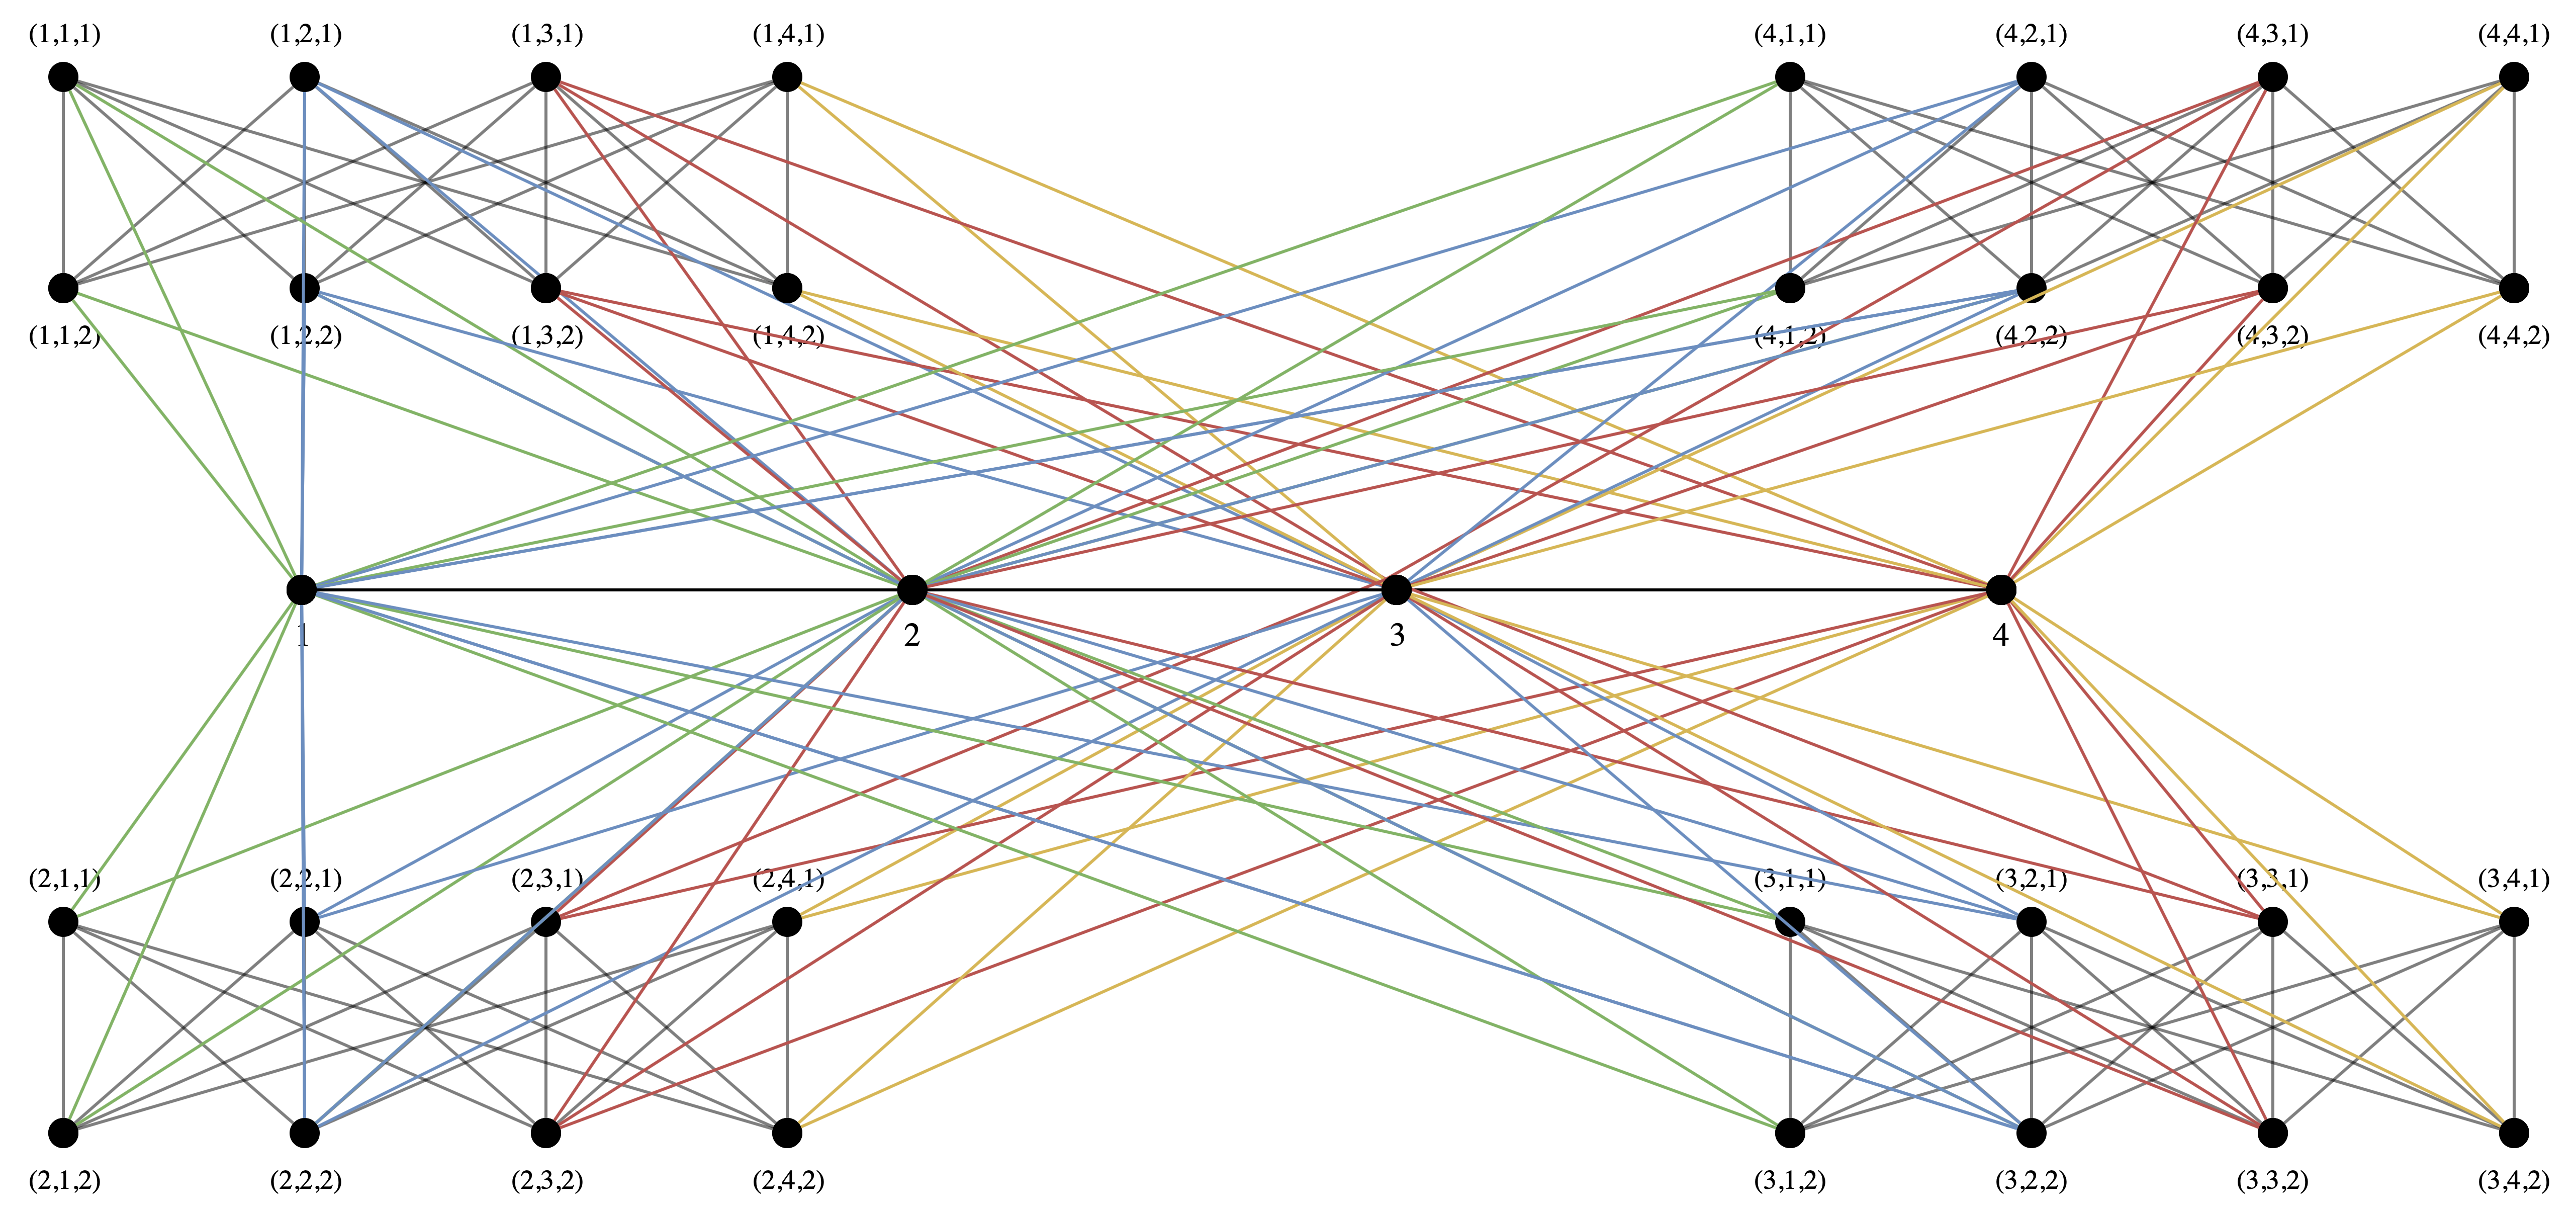
\includegraphics[width=0.9\linewidth]{fig/sec5.png}
			\caption{$H$ obtained from $P_4$, zombie player needs at least $\gamma(P_4) = 2$ zombies to win}
			\label{fig:p8}
		\end{figure}

		By having zombies on each vertex of $G$'s dominating-set, survivor will be captured on the first move and zombie
		player wins. Thus, $\zn(H) \leq \gamma(G)$. Now suppose we have zombies less than the domination number of
		graph: $\mathpzc{z} < \gamma(G)$. We prove survivor can avoid being captured.
		
		Since there are $n$ bipartite subgraphs, one of them is initially free of zombies. Further, since zombies are
		not dominating $G$, there will be a vertex $w \in V(G)$ with no zombies as its neighbors. Thus the survivor can
		safely start at vertex $(k,v = w,b = 1)$ (let $(k,v,b)$ denote the survivor's vertex).

		Zombies in $G$ (e.g. at vertex $u$) are at distance 2 from survivor $(u \rightarrow (k,u,3 - b) \rightarrow
		(k,v,b))$, which means after their move all of them should be at one of $(k,v,b)$'s neighbors, that is, $N_G[v]
		$ or, $ (k,1 \leq i \leq n,3 - b)$. Therefore, each zombie joining $B_k$ does not share the same partition as
		survivor's, since it has to be on one of its neighbors.
		
		On each survivor turn, assume that the survivor is at $(k,v,b)$ and zombies are either in $G$, or in $B_{(i \neq
		k)}$, or in $B_k$ at a vertex of the form $(k,j,3-b)$ (not in the same partition as survivor). Since there is a
		vertex $w \in G$ not being dominated by zombies, survivor should move to vertex $(k,w,3-b)$. Since the survivor
		is now sharing the same partition as all zombies in $B_k$, and $N_G[w]$ is empty of zombies, non of his
		neighbors is occupied by a zombie and survivor will be safe by following this strategy indefinitely.

		It is now proved that $\zn(H) = \gamma(G)$, thus the dominating-set problem is reduced to $\NPZ$.

	\end{proof}
\begin{thebibliography}{999}
	
	\bibitem{Fitz16}
	Fitzpatrick, Shannon L., J. Howell, Margaret-Ellen Messinger, and David A. Pike. ``A deterministic version of the
	game of zombies and survivors on graphs." Discrete Applied Mathematics 213 (2016): 1-12.
	\bibitem{Offner19}
	Offner, David, and Kerry Ojakian. ``Comparing the power of cops to zombies in pursuit-evasion games." Discrete
	Applied Mathematics (2019).
	\bibitem{West02}
	West, Douglas B. ``Introduction to Graph Theory." Prentice hall, (1996).
	\bibitem{Hopcroft07}
	J. E. Hopcroft, R. Motwani, and J. D. Ullman. ``Introduction to Automata Theory, Languages, and Computation.''
	Pearson Addison-Wesley, (2007).
	\bibitem{Bonato09}
	A. Bonato, P. Golovach, G. Hahn, and J. Kratochvıl, ``The capture time of a graph'', Discrete Mathematics 309 (2009), 5588–5595.
	\bibitem{Fomin10}
	Fomin, Golovach, Kratochvil, Nisse, ``Pursing fast robber in graphs", Theoretical Computer Science, 411 (2010) 1167 - 1181
\end{thebibliography}

\newpage
\appendix
\section{An example for zombie number of Cartesian product of two graphs} \label{CartesianProductExample}
\begin{example} $\zn(P_3 \square P_4 ) = 2$
\end{example}

\begin{figure}[h!]
	\centering
	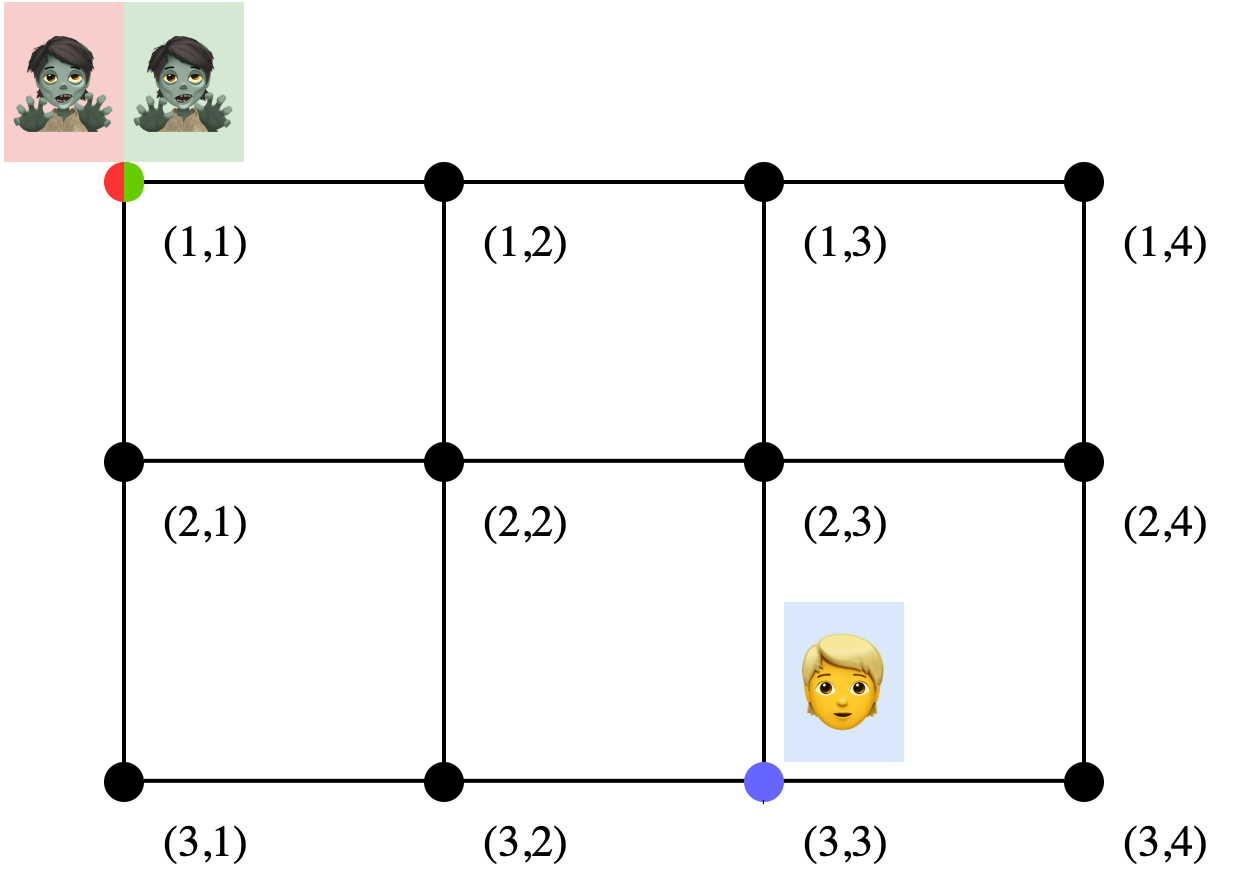
\includegraphics[width=0.5\linewidth]{fig/p34m1.png}
	\caption{$P_3 \square P_4$ and initial vertices}
	\label{fig:p3}
\end{figure}

It is easy to show that $\zn(P_3) = \zn(P_4) = 1$. On each of these path graphs, zombie's initial position could be any
vertex of the graph. For this example, we put the {\it G-zombie} and {\it H-zombie} ($G = P_3$ and $H = P_4$) both on
vertex $(1,1)$. We show the survivor with blue color, {\it H-zombie} with red, and {\it G-zombie} with green. {\it
G-zombie} will try to get to the same $G_{i}$ as survivor's which is $G_3$ using an {\it H-edge}. {\it H-zombie} will
try to get to $H_3$ (See figure \ref{fig:p4}).

\begin{figure}[h!]
	\centering
	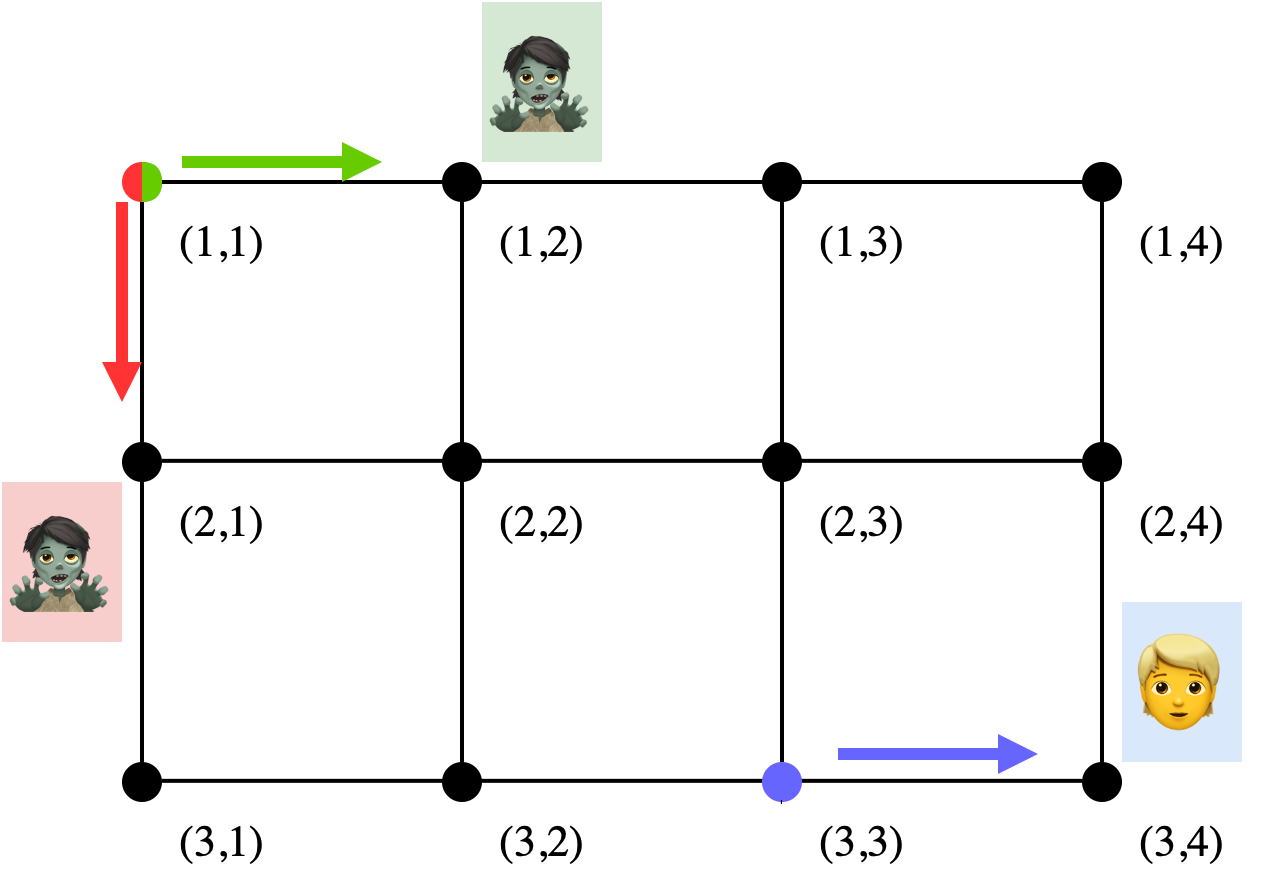
\includegraphics[width=0.5\linewidth]{fig/p34m2.png}
	\caption{First move of players}
	\label{fig:p4}
\end{figure}

After zombies' move the survivor must move. No matter what move he makes, either {\it G-zombie} has made itself closer
to $H_x$ or {\it H-zombie} has made itself closer to $G_y$. In this case, {\it H-zombie} got closer to $H_x$. Since
neither {\it H or G-zombie}s share $H_x$ or $G_y$ with the survivor, they will still try to achieve that (See figure \ref{fig:p5}).

\begin{figure}[h!]
	\centering
	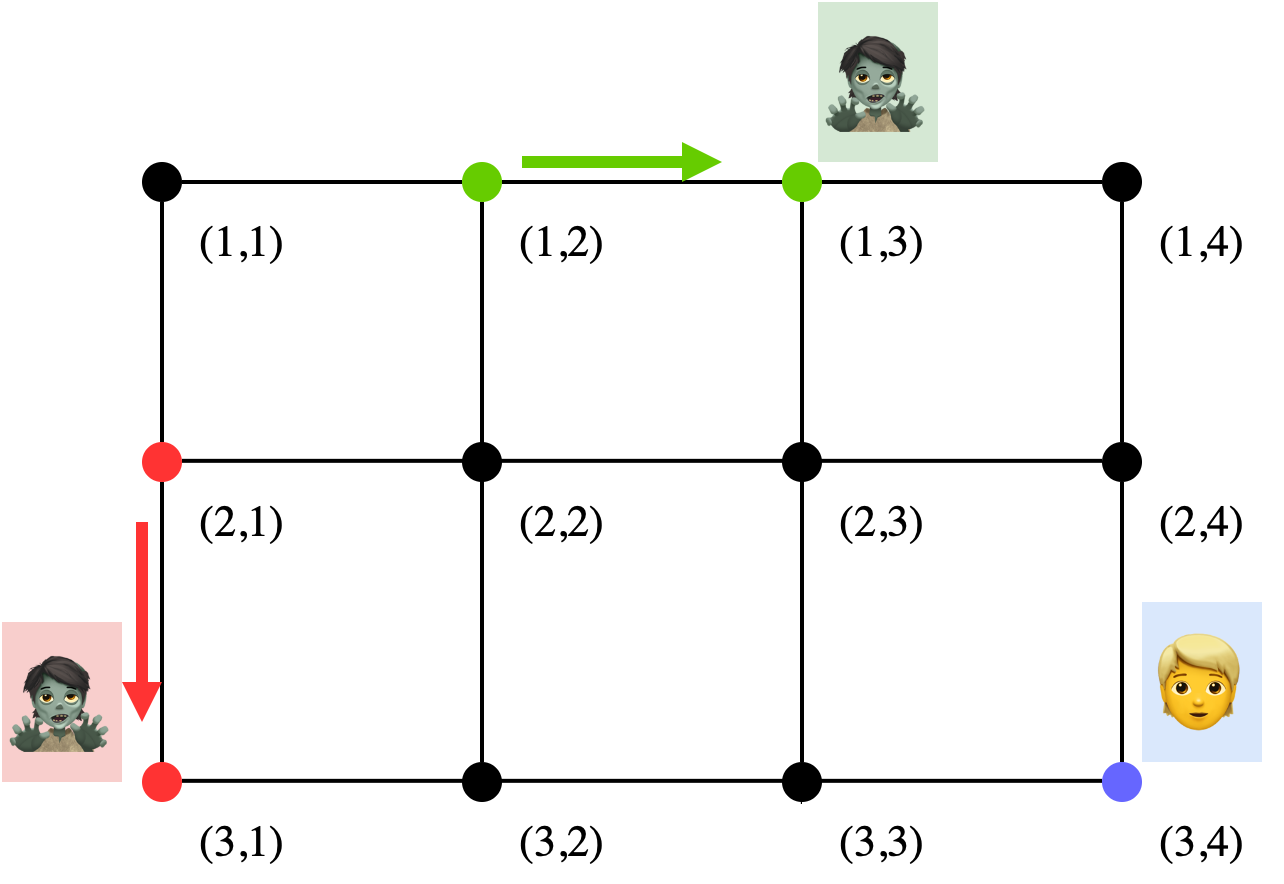
\includegraphics[width=0.5\linewidth]{fig/p34m3.png}
	\caption{Second move made by zombies, third in total}
	\label{fig:p5}
\end{figure}

Now {\it H-zombie} shares the same copy of $H$ as survivor and it is survivor's turn. If survivor moves to another
$H_i$, {\it H-zombie} will mimic the move. If survivor makes an {\it H-move}, {\it H-zombie} will do whatever it did on
a single $H$ for capturing the survivor. This means survivor cannot do infinite {\it H-move}s. Thus for him being able
to survive he has to do infinite {\it G-move}s, which again leads to {\it G-zombie} capturing him. For other moves, you
can see figure \ref{fig:p6}.

\begin{figure}[h!]
	\centering
	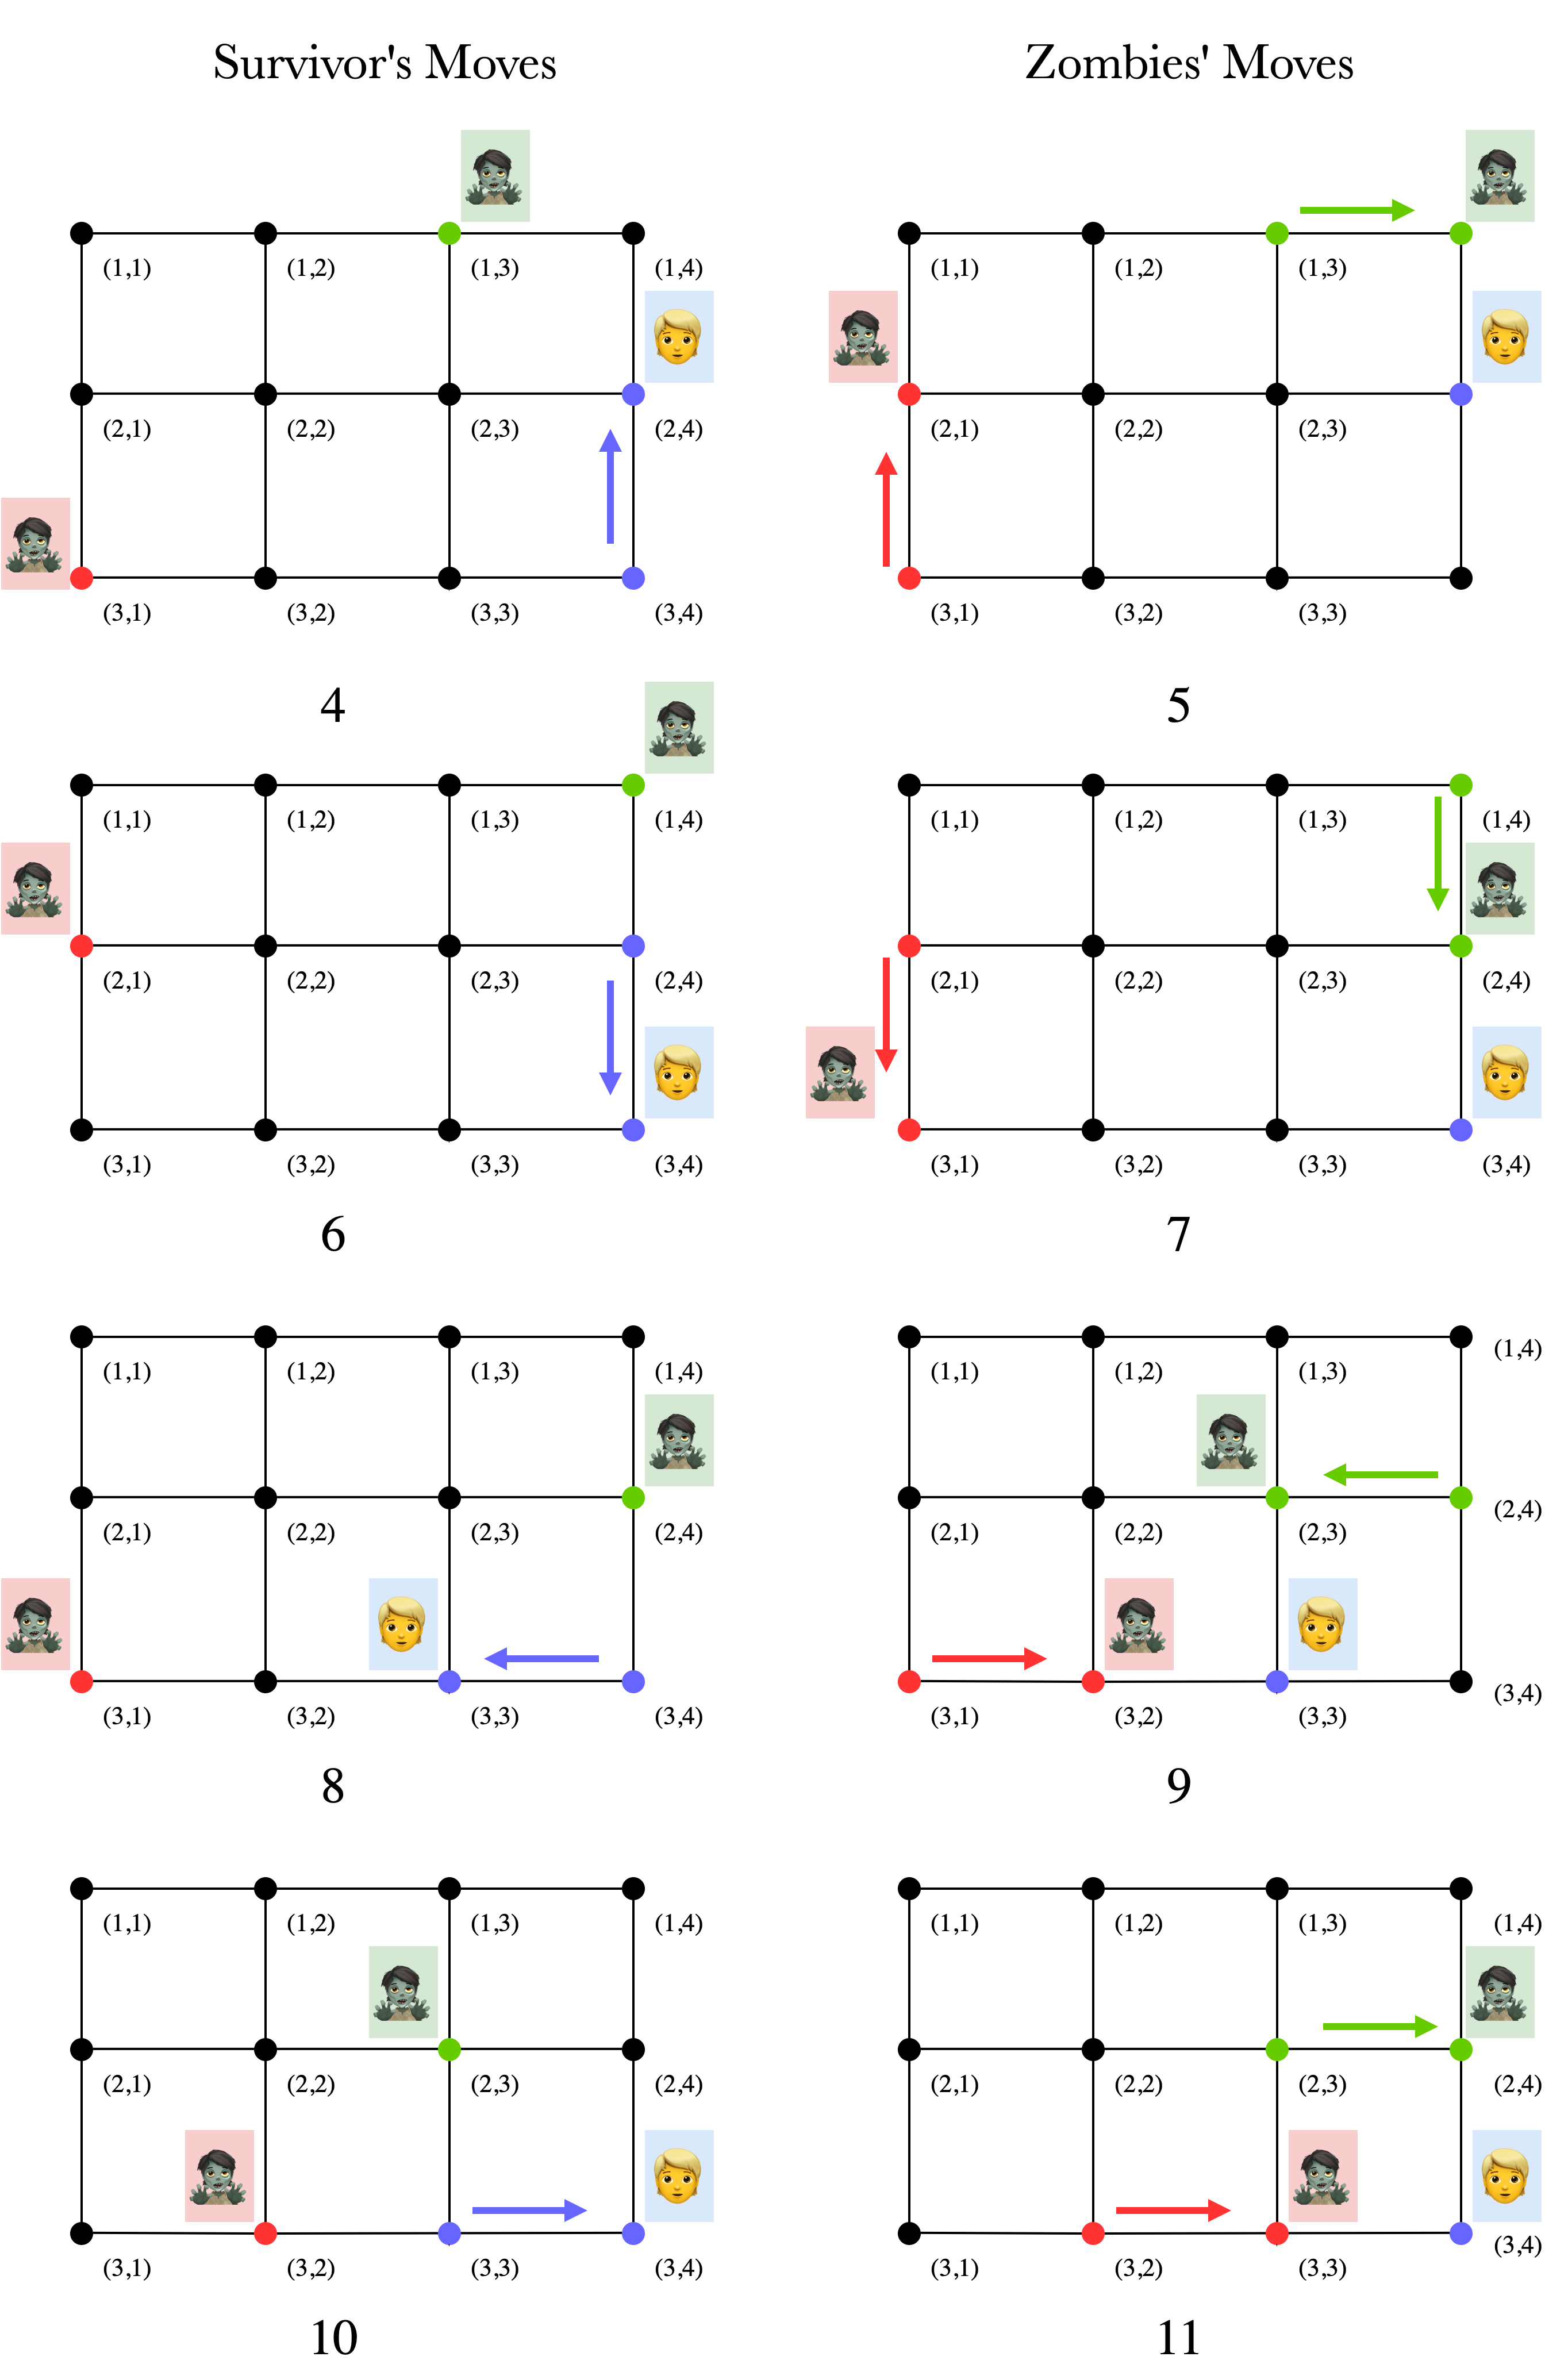
\includegraphics[width=1\linewidth]{fig/p34m6.png}
	\caption{Other moves made by players}
	\label{fig:p6}
\end{figure}

	
\end{document}